\documentclass[12pt]{article}
\usepackage{a4}
\usepackage[english]{babel}
\setlength{\parindent}{0.35cm}
\pagestyle{headings}
\usepackage{graphicx}
\usepackage{grffile}
%Multiple picture in one figure
%\usepackage{subfigure}
\usepackage{subfig}
\usepackage[utf8]{inputenc}
\usepackage{listings}
\usepackage{color}
\usepackage{wrapfig}
%Floating-Umgebungen
\usepackage{float}
%Math-Environment
\usepackage{amsmath}
\usepackage{amssymb}
\usepackage{bbm}
%Better SI-Units
\usepackage{siunitx}
%Using Appendix
\usepackage[title]{appendix}
%Using URL
\usepackage[hidelinks]{hyperref}
%Using Colored Tables
\usepackage{colortbl}
\newcommand{\gray}{\rowcolor[gray]{.90}}
\usepackage{esvect}
% Use fancy tables
\usepackage{tabularx}
% Build fancy tables
\usepackage{booktabs}
% Configure enumeration
\usepackage{enumitem}
%Configure geometry
\usepackage{geometry}
\geometry{
	a4paper,
	left=3cm,
	right=3cm,
	top=3cm,
	bottom = 3cm,
	}

\lstset{
	language=C++,
	basicstyle=\small\ttfamily,
	keywordstyle=\color{blue}\ttfamily,
	stringstyle=\color{red}\ttfamily,
	commentstyle=\color{green}\ttfamily,
	morecomment=[l][\color{magenta}]{\#},
}


\usepackage{amsthm}

\renewcommand\qedsymbol{$\blacksquare$}
\newtheorem{theorem}{Theorem}[section]

\begin{document}
	
	\title{
		\textbf{\huge{CSE 446: Machine Learning Winter 2018 }} \\[2cm]
		\LARGE{Assignment 3}\\[1cm]
	}
	\author{from \\ Lukas Nies \\ University of Washington}
	\date{02/22/18}
	\clearpage\maketitle\thispagestyle{empty}
	\newpage

	\tableofcontents
	\setcounter{page}{0}
	\newpage
	
	% To start with section 1 labeled as section 0
	\setcounter{section}{-1}
	

\section{Policies}

\subsection{List of Collaborators}

My collaborator was Edith Heiter (discussed Problem 2 and 4). The development of the answers though was completely independent and individually.

\subsection{List of Acknowledgments}

None.

\subsection{Policies}

I have read and understood these policies.

\newpage

\section{Problem: Linear Regression on MNIST}

\subsection{Closed Form Estimator}

\begin{enumerate}
	\item If one runs the Closed Form Estimator with $\lambda = 0$ one encounters trying to invert a singular matrix ($X^TX$) which is not possible per definition since the determinant is $\det(X^TX)=0$. The matrix is therefore not invertible. To avoid this we introduce a regularization by adding the term $\lambda\mathbbm{1}_d$. This is intuitively clear by considering the data itself: one digit consists of $28\times 28$ pixels where most pixels (at the edges and in the corners) don't carry any information about the digit itself. When calculating $X^TX$ we get the same result: we have more "dimensions" than information for those "dimensions". In mathematical terms: $X^TX$ is underdetermined.
	\item For this part a grid search was implemented to search for different values of $\lambda$ and the threshold to optimize the performance on the development set:
		\begin{enumerate}[label=(\alph*)]
			\item The best result was found with $\lambda=101$ and a threshold of $0.4$. The grid search ran for $\lambda$ from 1 to 250, the treshold ran from 0.1 to 1.0.
			\item The average squared error using the parameters stated above is as follows:
				\begin{itemize}
					\item $\text{Training error}=0.09165$
					\item $\text{Development error}=0.01907$
					\item $\text{Test error}=0.02132$
				\end{itemize}
			\item The misclassification error using the parameters stated above is as follows:
			\begin{itemize}
				\item $\text{Training error}=1.88\%$
				\item $\text{Development error}=1.64\%$
				\item $\text{Test error}=2.30\%$
			\end{itemize}
		\end{enumerate}
	\item Samples with large values (far off the mean of the rest of the data points) have a strong influence on linear polynomial functions fitted through regression. This leads to large misclassification on most of the data points. 
\end{enumerate}

\subsection{Linear regression using gradient descent}

\begin{enumerate}
	\item The proof is as follows:
		\begin{align*}
			\frac{\partial \mathcal{L}_w}{\partial w} &= \frac{\partial}{\partial w} \left( \frac{1}{N} \sum_{n=1}^{N} \frac{1}{2} \left( y_n - w^Tx_n \right)^2 + \frac{\lambda}{2} \lVert w \rVert^2 \right) \\
			&= \frac{1}{N} \sum_{n=1}^{N} \left( -\frac{2x_n}{2} \right) \left( y_n - w^Tx_n \right) + \left( \frac{2\lambda}{2} \textbf{w}  \right) \\
			&= -\frac{1}{N} \sum_{n=1}^{N} \left( y_n - \hat{y}_n \right) x_n + \lambda \textbf{w}
		\end{align*}
	\item We can rewrite this as a matrix expression:
		\begin{align*}
			\frac{\partial \mathcal{L}_w}{\partial w} = -\frac{1}{N} \sum_{n=1}^{N} \left( y_n - \hat{y}_n \right) x_n + \lambda \textbf{w} = - \frac{1}{N} X^T \cdot \left( Y - \hat{Y} \right) + \lambda \textbf{w}
		\end{align*}
	\item Stepsizes $ 10^{-3} \leq \eta \leq 10^{-2} $ worked well for this problem. For the error rate see figure \ref{fig:1.2}. For generating the plots, $\lambda=1$ and $\eta=10^{-2}$ were chosen.
		\begin{figure}[h!]
			\centering
			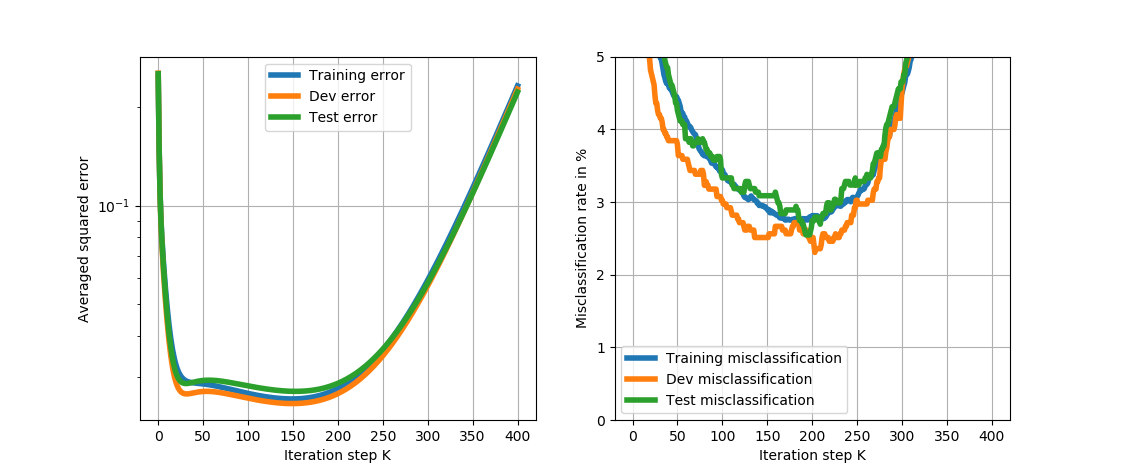
\includegraphics[width=\linewidth]{./Problem_1/Problem_1.2_10-2.png}
			\caption{Plot of averaged squared errors (left, note the logarithmic vertical axis) and misclassification loss in percent (right). For generating the plots, $\lambda=1$ and $\eta=10^{-2}$ were chosen.}
			\label{fig:1.2}
		\end{figure}
\end{enumerate}

\subsection{Linear Regression Using Stochastic Gradient Descent}


\newpage


%\chapter*{Bibliography}
\addcontentsline{toc}{chapter}{Bibliography}%	

\bibliographystyle{unsrt}
\bibliography{./bib}





\end{document}  